% !TEX root = ../document.tex
\section{Blockchain in der Praxis am Beispiel Multichain}
\label{sec:Praxis}
Im nun folgenden Praxisteil soll eine Blockchain aufgesetzt, verwaltet und mit dieser verschiedene Aktionen durchgeführt werden, die einige im Theorieteil vorgestellten Aspekte praktisch vorführen.

\subsection{Installation, Einrichtung und Generierung der Blockchain}
\label{subsec:inst}
Zur Realisation des Praxisteils wird MultiChain verwendet. MultiChain ist eine offene Software mit deren Hilfe schnell und einfach Blockchains erstellt und verwaltet werden können.\footnote{https://www.multichain.com/} Zudem bietet MultiChain einen eigens entwickelten Web-Explorer, um die Blockchain leichter nachvollziehen zu können.\footnote{https://github.com/MultiChain/multichain-explorer} Um die Dezentralität der Blockchain darzustellen, müssen mindestens zwei Nodes die Blockchain verwenden. Um dies allerdings auf einem Computer realisieren zu können und um den Stand des Praxisteils exportierbar zu machen, wird der Praxisteil mit Hilfe zweier virtueller Maschinen verwirklicht. Auf der ersten virtuellen Maschine wird die Blockchain erstellt (im Folgenden Server genannt), sodass die andere virtuelle Maschine (im Folgenden Client genannt) sich dieser Blockchain später anschließen kann.

Um die Blockchain nun auf dem Server einzurichten, muss zunächst MultiChain installiert werden. MultiChain ist sowohl für Linux als auch für Windows und Mac verfügbar. Da beide virtuellen Maschinen allerdings eine Linux-Distribution (Ubuntu) besitzen, wird lediglich auf die Installation für Linux eingegangen. Dazu muss zunächst von der MultiChain-Webseite eine Datei mit den Sourcen heruntergeladen werden, die dann entpackt werden muss. Um MultiChain einfach über das Terminal bedienbar zu machen, werden zudem drei Dateien in den Ordner /usr/local/bin verschoben. Diese Schritte können einfach mittels folgender Zeilen im Terminal durchgeführt werden\footnote{https://www.multichain.com/download-install/}:

\begin{lstlisting}[frame=single]
su (enter root password)
cd /tmp
wget https://www.multichain.com/download/multichain-1.0.4.tar.gz
tar -xvzf multichain-1.0.4.tar.gz
cd multichain-1.0.4
mv multichaind multichain-cli multichain-util /usr/local/bin
exit
\end{lstlisting}

Nachdem MultiChain nun installiert ist, kann die Blockchain erstellt werden. Jede Blockchain muss zudem benannt werden. Für dieses Praxisbeispiel wird die Blockchain „db“ genannt. Mittels folgenden Kommandos kann die Blockchain erstellt werden.

\begin{lstlisting}[frame=single]
multichain-util create db
\end{lstlisting}

Dadurch wird in dem Verzeichnis ~/.multichain nun ein neuer Ordner mit dem Namen der Blockchain angelegt, der die gesamte Blockchain inklusive Daten und Einstellungen enthält. Als nächstes können, falls gewollt, die Parameter der Blockchain angepasst werden. Diese befinden sich in der Datei params.dat des jeweiligen Blockchain-Ordners und können in diesem Fall mittels folgenden Kommandos bearbeitet werden.

\begin{lstlisting}[frame=single]
sudo nano ~/.multichain/db/params.dat
\end{lstlisting}

Eine Liste aller verfügbaren Parameter und deren Bedeutung befindet sich ebenfalls auf der Webseite von MultiChain.\footnote{https://www.multichain.com/developers/blockchain-parameters/} Erwähnenswert in Bezug auf Kryptowährungen ist hier der Parameter initial-block-reward mittels dessen eingestellt werden kann, wie viel Währung ein Node als Belohnung für das erfolgreiche Validieren eines Blocks erhält.

Die Blockchain ist nun erstellt und eingerichtet allerdings noch nicht generiert, d. h. sie besitzt noch keinerlei Blöcke und entsprechend keine Daten. Um die Blockchain nun also zu generieren, muss ein erster Block vom Server validiert werden. Um die Validierung und somit das Errechnen eines gültigen Hashes für den nächsten Block zu starten, wird in diesem (bezogen auf diese Blockchain) folgendes Kommando verwendet.

\begin{lstlisting}[frame=single]
	multichaind db -daemon
\end{lstlisting}

Sobald der erste Block validiert ist, ist die Blockchain generiert.

\subsection{Installation und Einrichtung des MultiChain-Explorers}
\label{subsec:trans-erstellung}
Um die Blockchain auch übersichtlich und verständlich betrachten zu können wird nun der von MultiChain zur Verfügung gestellte Explorer installiert. Die Sourcen für den Explorer befinden sich in einem GitHub-Repository von MultiChain und können (sofern Git auf dem Server installiert ist) mittels folgenden Kommandos heruntergeladen werden:

\begin{lstlisting}[frame=single]
git clone https://github.com/MultiChain/multichain-explorer
\end{lstlisting}

Damit der Explorer lauffähig ist, sind allerdings einige zusätzlichen Programme notwendig, die über folgende Kommandos heruntergeladen und installiert werden können:

\begin{lstlisting}[frame=single]
sudo apt-get install sqlite3 libsqlite3-dev
sudo apt-get install python-dev
sudo apt-get install python-pip
sudo pip install -upgrade-pip
sudo pip install pycrypto
\end{lstlisting}

Als nächstes muss in den nun angelegten Ordner multichain-explorer gewechselt und dort das Skript setup.py mit dem Argument install ausgeführt werden, um den Explorer zu installieren. 

\begin{lstlisting}[frame=single]
cd multichain-explorer
sudo python setup.py install
\end{lstlisting}

Als nächstes muss der Explorer mit der generierten Blockchain kommunizieren können, um die Daten dieser später anzeigen zu können. Jede Blockchain besitzt einen sog. RPC-Port, der in der Datei params.dat im Ordner der Blockchain festgelegt ist. Damit die Blockchain mit dem Explorer kommunizieren kann, wurde bereits beim Erstellen dieser die Datei multichain.conf im Ordner der Blockchain angelegt. In diese Datei muss nun der RPC-Port eingetragen werden. Dies lässt sich einfach über folgende Kommandos realisieren (wobei AUSGEGEBENER\_PORT entsprechend ersetzt werden muss):

\begin{lstlisting}[frame=single]
cd ~/.multichain/db
grep rpc params.dat
echo "rpcport=AUSGEGEBENER_PORT" >> multichain.conf
\end{lstlisting}

Abschließend muss der Explorer noch mit der Blockchain verknüpft werden. Hierzu muss zunächst wieder in den Ordner multichain-explorer navigiert werden. Es muss nun eine Konfigurationsdatei eigens für die erstellte Blockchain angelegt und konfiguriert werden. MultiChain-Explorer bietet hierzu eine vorgefertigte Konfigurationsdatei (chai1.example.conf) die einfach kopiert und unter dem Namen der Datenbank (db.conf) gespeichert werden kann. Innerhalb der Datei können bzw. müssen nun folgende Parameter eingestellt werden:

\begin{table}[h]
	\begin{tabular}{|l|l|}
		\hline 
		\textbf{Parameter} & \textbf{Beschreibung} \\ 
		\hline 
		port & Port, über den die Seite im Browser erreichbar sein soll \\ 
		\hline 
		host & IP des Gerätes, das den Explorer aufrufen können soll (0.0.0.0 für alle Geräte) \\ 
		\hline 
		dirname & Absoluter Pfad zum Ordner der Datenbank (hier: ~/.multichain/db) \\ 
		\hline 
		chain & Name der Blockchain, der im Explorer angezeigt werden soll \\ 
		\hline 
		connect-args & Speicherort der Explorer-Datenbank (hier: db.explorer.sqlite) \\ 
		\hline 
	\end{tabular}
	\caption{Konfigurierbare Parameter der Explorer-Blockchain-Verbindung}
\end{table}

Nachdem die Parameter entsprechend angepasst wurden, kann die Datei mit der Tastenkombination STRG + X verlassen werden, wobei auf die Nachfrage, ob die Änderungen gespeichert werden sollen mit Y + Enter und danach der Dateiname mit Enter bestätigt werden müssen.

Nun kann der Explorer mit folgendem Kommando gestartet werden:

\begin{lstlisting}[frame=single]
sudo python -m Mce.abe -config db.conf
\end{lstlisting}

Der Explorer liest dann zunächst die bislang getätigten Transaktionen und validierten Blöcke in die eigene Datenbank ein. Der Explorer kann dann über die Adresse des Servers und dem angegebenen Port aufgerufen werden (s. Abbildung \ref{fig:1}).

\begin{figure}[h]
	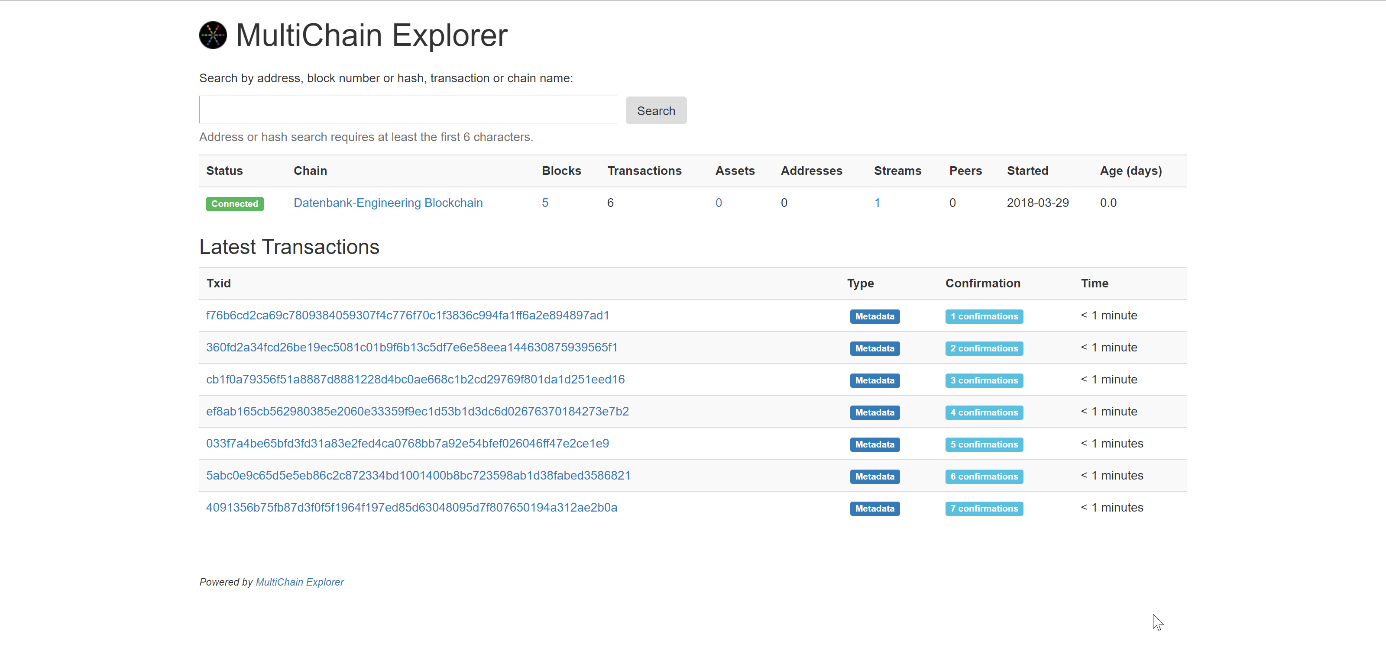
\includegraphics[width=\textwidth]{1.png}
	\caption{Startseite des Explorer}
	\label{fig:1}
\end{figure}

\subsection{Anbinden eines zweiten Knoten an die Blockchain}
\label{subsec:trans-erstellung-mit-daten}
Um nun unseren Client zum zweiten Knoten der Blockchain zu machen, müssen wir auch auf diesem zunächst MultiChain installieren. Voraussetzung für die Verbindung ist nun, dass sich die beiden Computer (bzw. hier die beiden virtuellen Maschinen) im selben Netzwerk befinden. Als der Server als Knoten der Blockchain gestartet wurde, wurde im Terminal des Servers folgendes ausgegeben:

\begin{figure}[h]
	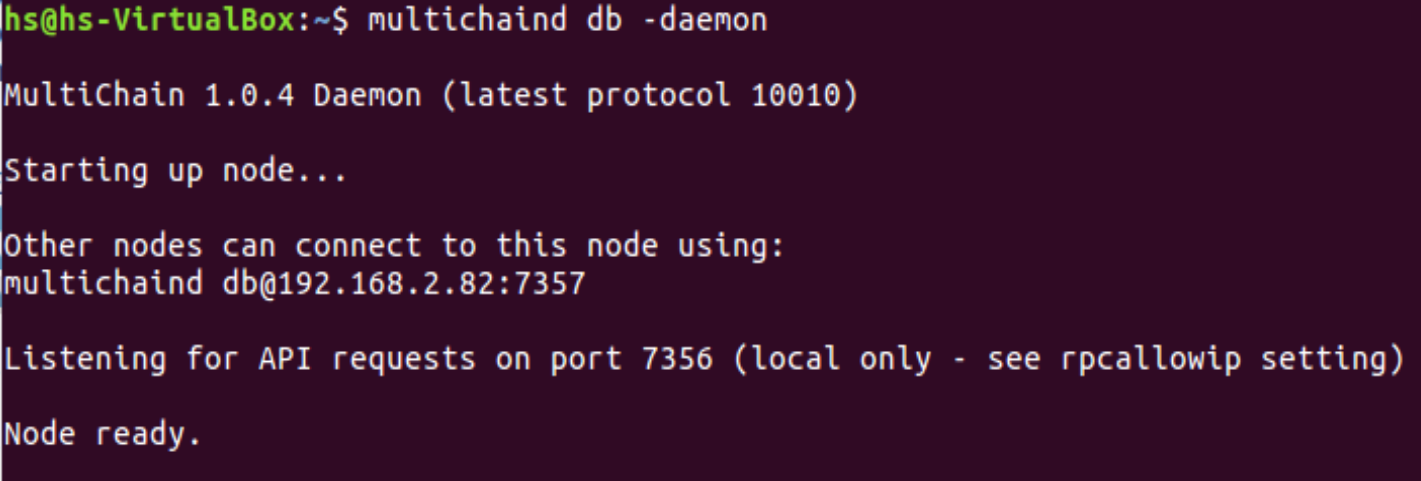
\includegraphics[width=\textwidth]{2.png}
	\caption{Ausgabe des Kommandos multichaind db -daemon im Terminal des Servers}
	\label{fig:2}
\end{figure}

Hier wird mitgeteilt, wie man sich mit anderen Computern im selben Netzwerk mit der Blockchain verbinden kann. Dazu muss man lediglich den Befehl multichaind eingeben gefolgt von dem Namen der Blockchain, einem @-Zeichen, der IP des Servers, einem Doppelpunkt und einem gesetzten Port. In diesem Falle setzt sich daraus folgendes Kommando zusammen:

\begin{lstlisting}[frame=single]
multichaind db@192.168.2.82:7357
\end{lstlisting}

Wenn dieses Kommando nun im Terminal des Clients eingegeben wird, erscheint allerdings ein Hinweis, dass Blockchain selbst zwar empfangen und erfolgreich auf dem Client initialisiert wurde, der Client nicht die nötigen Rechte zum Verbinden der Blockchain besitzt.

\begin{figure}[h]
	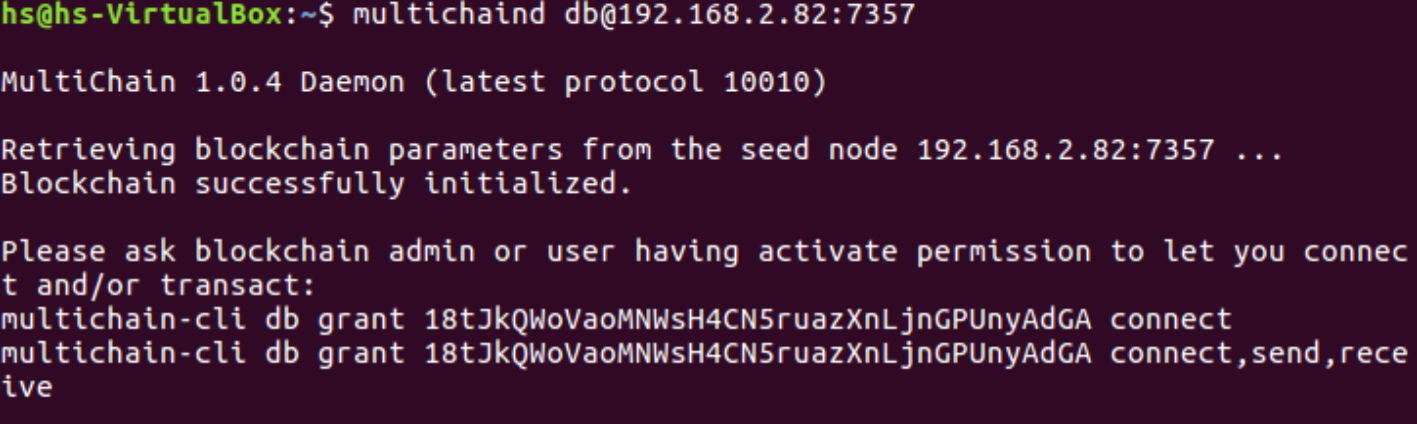
\includegraphics[width=\textwidth]{3.png}
	\caption{Initialisierung der Blockchain auf dem Client}
	\label{fig:3}
\end{figure}

MultiChain stellt eine Blockchain generell so ein, dass sich niemand ohne explizites Recht mit einer Blockchain verbinden kann. Dies kann allerdings vor der Generierung der Blockchain über den Parameter anyone-can-connect in der params.dat der jeweiligen Blockchain angepasst werden. Neben der Meldung über die fehlenden Rechte zeigt das Terminal des Clients allerdings auch direkt das Kommando an, das auf dem Server eingegeben werden muss, um dem Client die Rechte zum Verbinden zu geben:

\begin{lstlisting}[frame=single]
multichain-cli db grant 18tJkQWoVaoMNWsH4CN5ruazXnLjnGPUnyAdGA connect
\end{lstlisting}

Auffällig ist hierbei die lange, zufallsgenerierte Zeichenkette. MultiChain vergibt jedem Knoten eine einzigartige ID und die hier angezeigte ID ist die ID, die für den Client generiert wurde. Nachdem wir das Kommando im Terminal des Servers eingegeben haben, kann sich der Client mit der Blockchain verbinden und als Knoten gestartet werden.

Vorher sollen dem Client allerdings zusätzlich die Rechte zum Validieren von Blöcken und Tätigen von Transaktionen gegeben werden. Dazu wird folgendes Kommando benötigt:

\begin{lstlisting}[frame=single]
multichain-cli db grant 18tJkQWoVaoMNWsH4CN5ruazXnLjnGPUnyAdGA mine,send,receive
\end{lstlisting} 

Bevor der Knoten nun gestartet wird, soll allerdings noch ein Blick in das Verzeichnis ~/.multichain auf dem Client geworfen werden. In diesem befindet sich bereits der Ordner der installierten Blockchain db. Wechselt man in den Ordner der Blockchain und und betrachtet den Inhalt, beinhaltet dieser bereits einige generelle Dateien die Blockchain. Vergleicht man den Ordner allerdings mit demselben Ordner auf dem Server, sieht man, dass der Server sowohl mehr Dateien als auch mehr Ordner beinhaltet. Teilweise sind dies solche, die lediglich der Server als Ersteller der Blockchain besitzt, teilweise sind dies wie z. B. der Ordner wallet allerdings auch die Transaktionen bzw. Daten der Blockchain. 

\begin{figure}[h]
	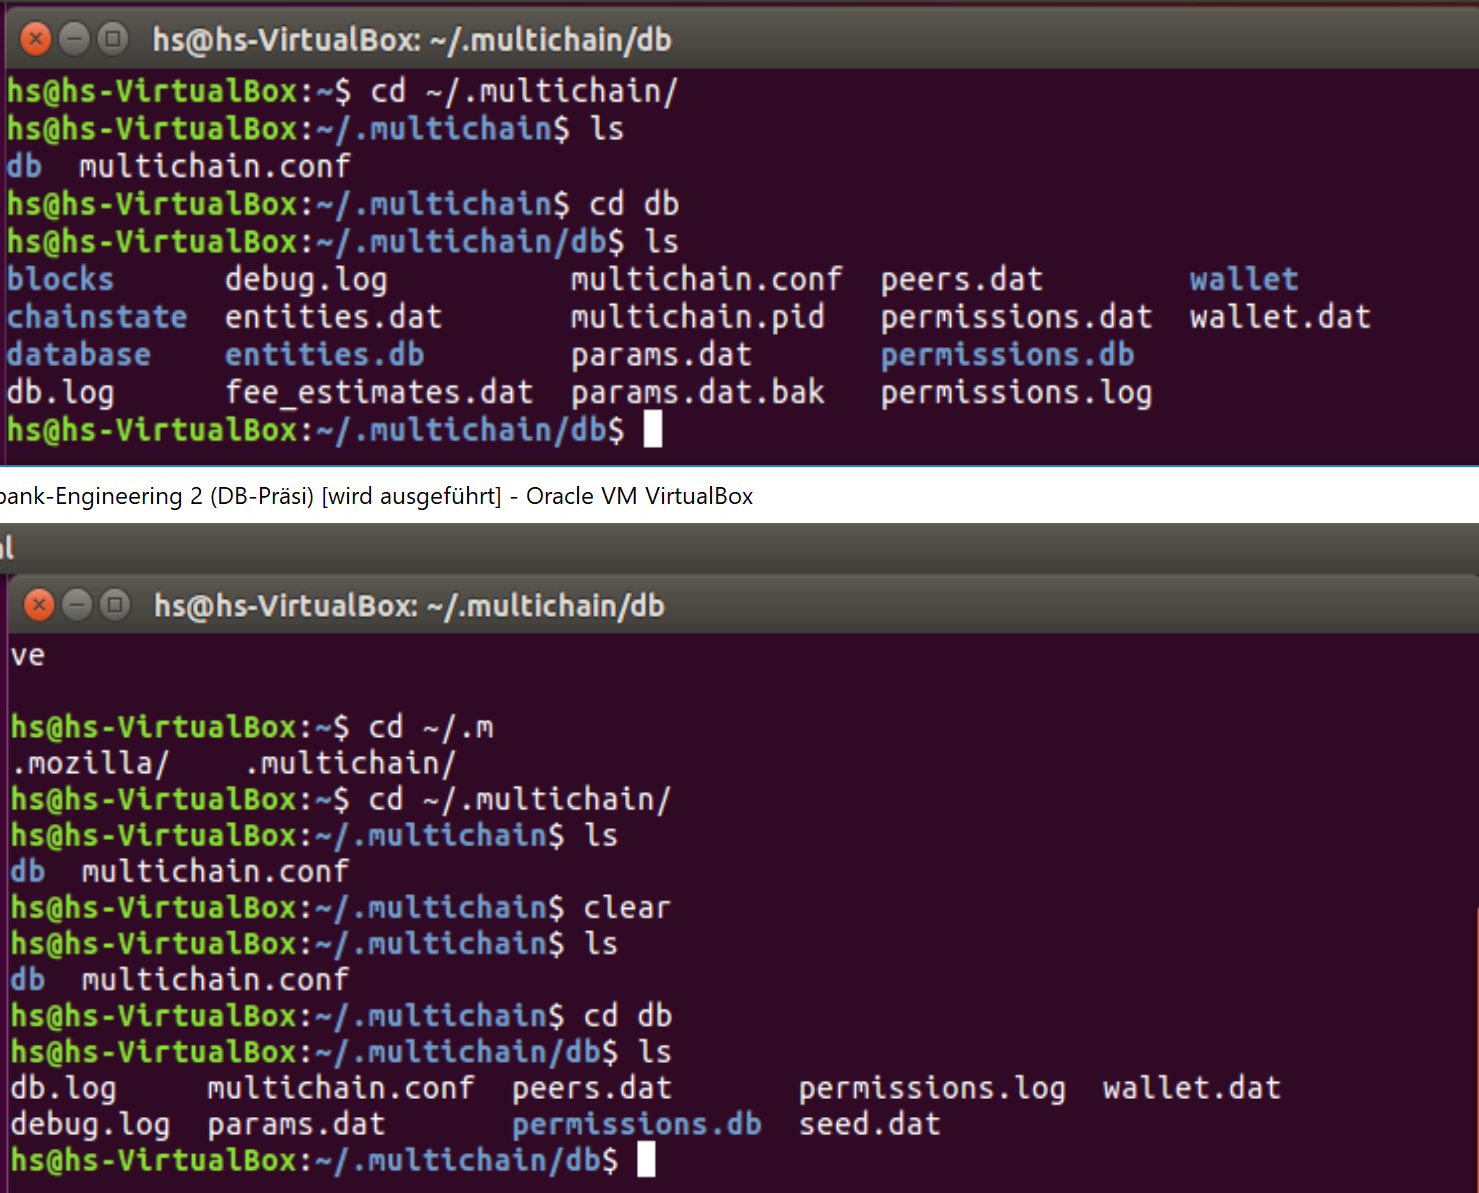
\includegraphics[width=\textwidth]{4.png}
	\caption{Vergleich des ~/.multichain/db-Ordners auf dem Server und dem Client}
	\label{fig:4}
\end{figure}

Um den Client nun als Knoten der Blockchain zu starten, wird dasselbe Kommando wie auf dem Server verwendet (multichaind db -daemon). An dieser Stelle wird nun die Dezentralität der Blockchain hervorgehoben: der Client empfängt nun alle Daten der Blockchain (Blöcke, Transaktionen, …), sodass alle Daten der Blockchain auf beiden Knoten liegen. Betrachtet man bspw. den Ordner wallet wird deutlich, dass beide Knoten alle Transaktionen beinhalten. Sobald neue Transaktionen hinzukommen, erhalten beide Knoten diese.

\begin{figure}[h]
	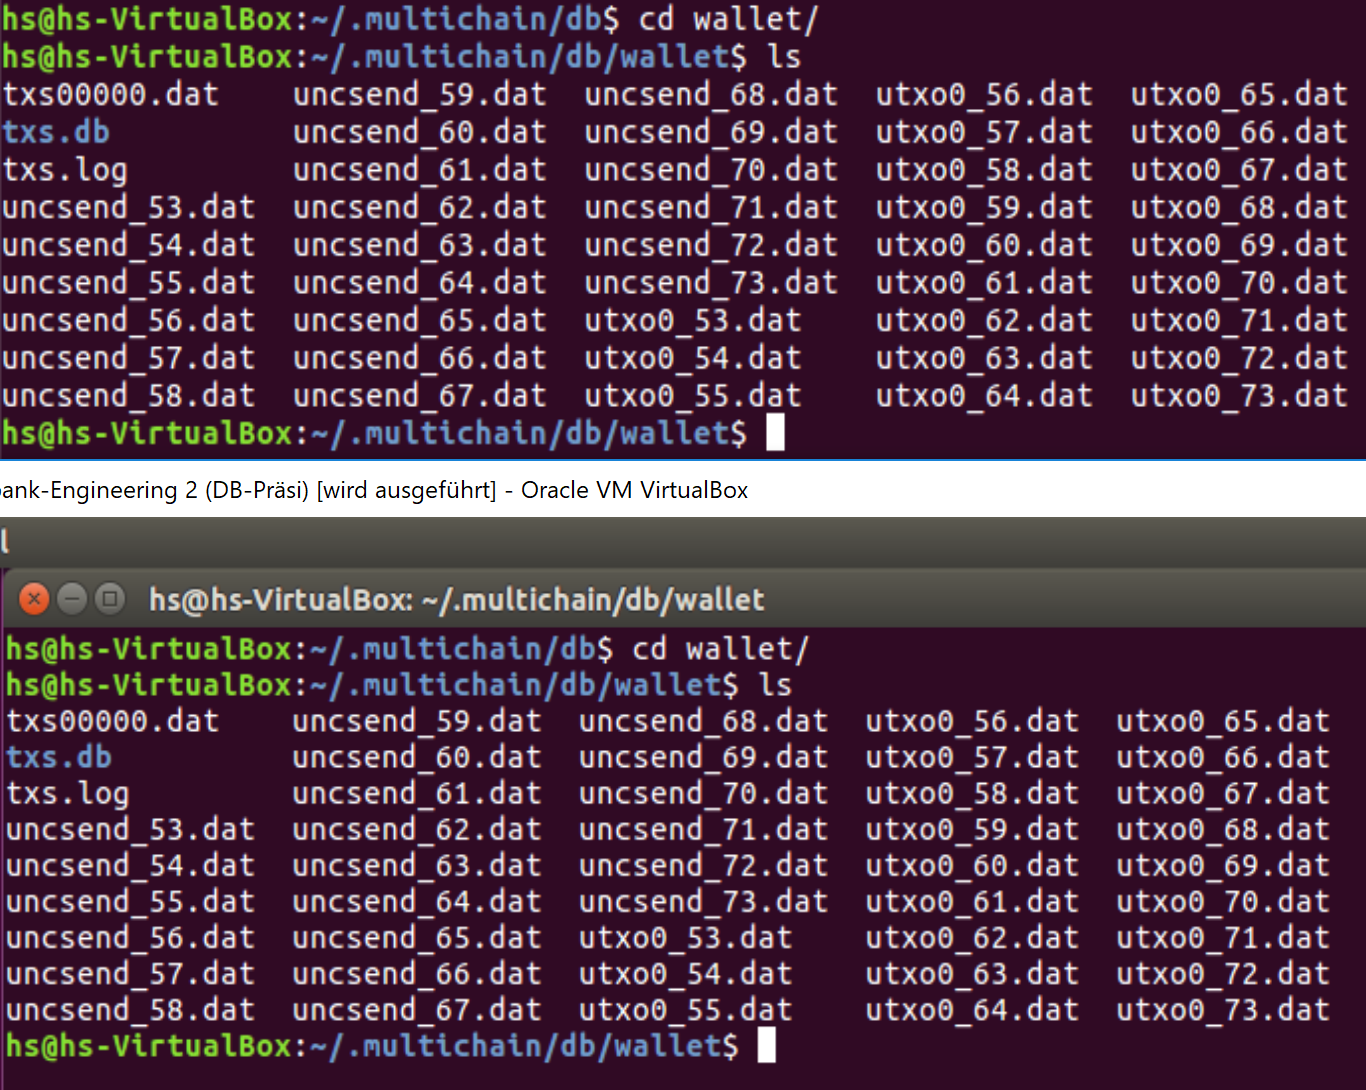
\includegraphics[width=\textwidth]{5.png}
	\caption{Vergleich des wallet-Ordners auf dem Server und dem Client}
	\label{fig:5}
\end{figure}

\subsection{Betrachtung der Blockchain im Explorer}
Beide Knoten sind nun am validieren der Blöcke. Dies lässt sich über den Explorer verfolgen. Wird die Startseite (s. Abbildung \ref{fig:1}) betrachtet, wird die Blockchain mit dem in der Datei db.conf angegebenen Namen angezeigt. Darunter werden zudem die letzten getätigten Transaktionen angezeigt. Wird nun neben dem Namen der Blockchain auf die Anzahl der Blöcke geklickt, gelangt man zur Übersicht der Blöcke der Blockchain (s. Abbildung \ref{fig:6}).

\begin{figure}[h]
	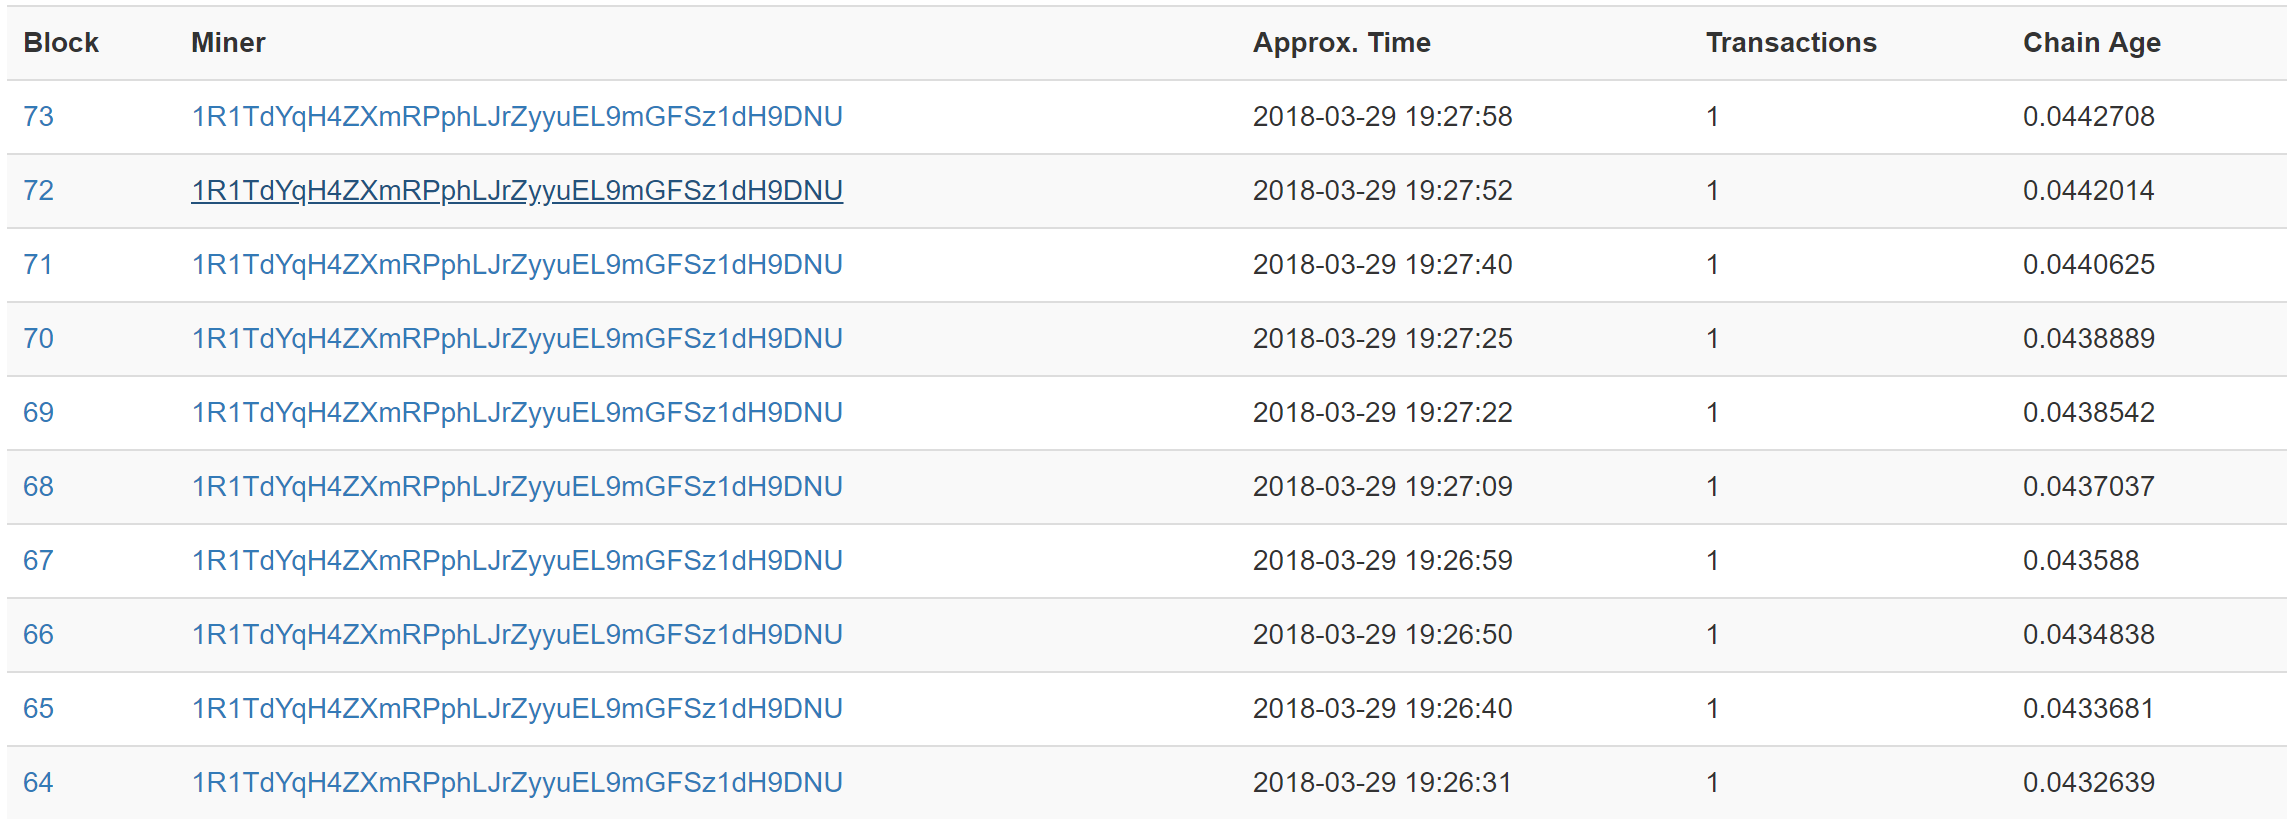
\includegraphics[width=\textwidth]{6.png}
	\caption{Übersicht der Blöcke der Blockchain}
	\label{fig:6}
\end{figure}

In der Liste wird für jeden Block folgendes angezeigt: die Nummer des Blocks in der Blockchain, die ID des Knotens, der diesen Block validiert hat, der Validierungszeitpunkt, die Anzahl der Transaktionen, die der Block beinhaltet bzw. validiert hat und das Alter der Blockchain zum Zeitpunkt der Validierung des Blocks in Tagen. Auffällig ist hierbei, dass die Blöcke bislang alle lediglich eine Transaktion beinhalten. Dies ist darauf zurückzuführen, dass die einzigen Transaktionen, die bislang ausgeführt wurden, die Gewinnausschüttung der Belohnung für das Validieren eines Blockes ist. Wird nun auf die Zahl eines Blocks geklickt, gelangt man zur Übersicht des Blocks (s. Abbildung \ref{fig:7}).

\begin{figure}[h]
	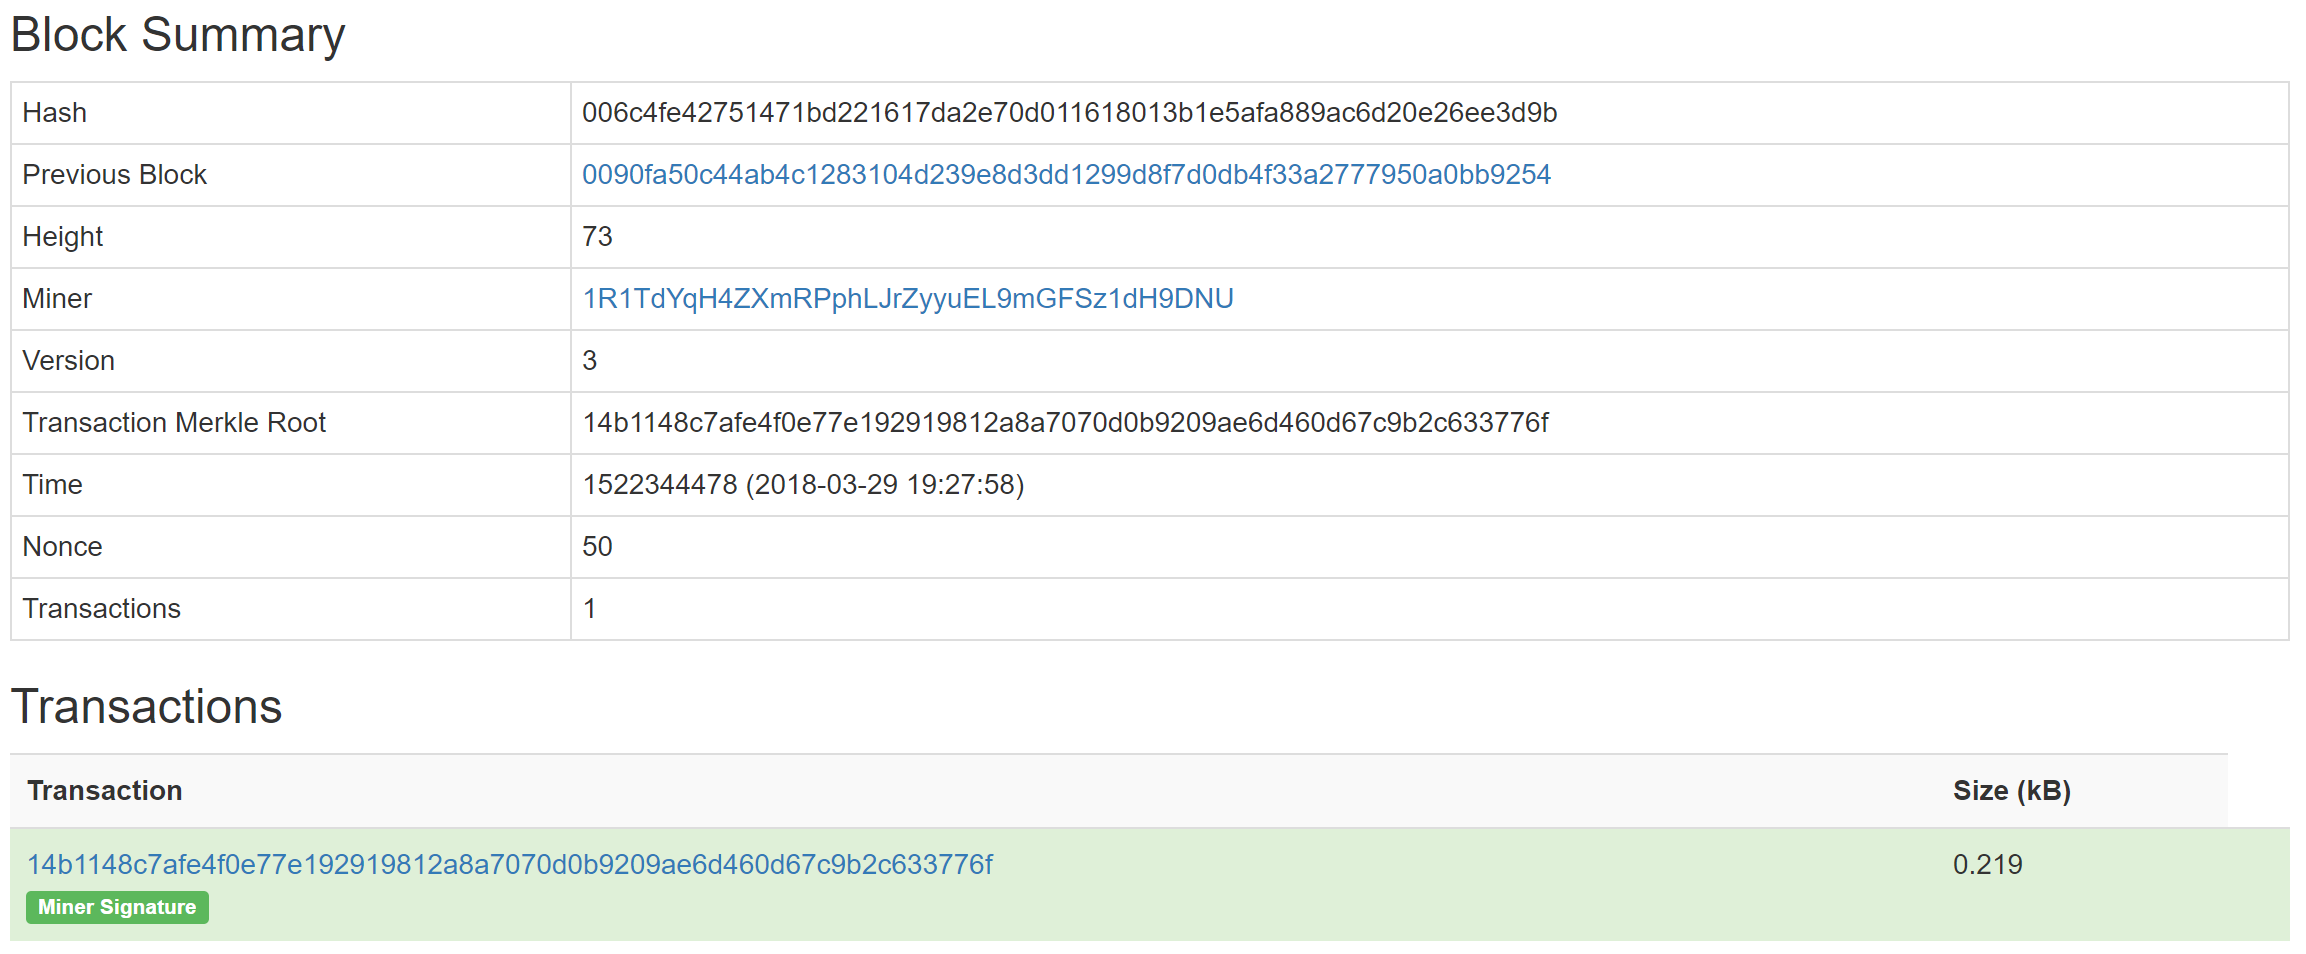
\includegraphics[width=\textwidth]{7.png}
	\caption{Ansicht eines Blocks im Explorer}
	\label{fig:7}
\end{figure}

In der Übersicht sieht man eine Liste mit Eigenschaften des Blocks und darunter die beinhalteten Transaktionen. In der Liste befindet sich zunächst der Hash des Blocks, der als gültiger Hash zum Validieren des Blocks errechnet worden ist. Bei MultiChain-Blockchains ist standardmäßig die Regelung eingestellt, dass ein Hash lediglich gültig ist, wenn er mindestens zwei Nullen voranstehen hat. Des Weiteren beinhaltet die Liste den Hash des vorherigen Blocks. Sobald ein nächster Block validiert wurde, wird zudem der Hash des nächsten Blocks eingetragen. Hier wird deutlich, wie die Blöcke verkettet sind und, dass eine entsprechend durch eine Änderung eines Blockes die Hash-Werte aller folgenden Blöcke neu berechnet werden müssten. Der Wert „Height“ zeigt die Nummer des Blocks in der Blockchain an. Darunter befindet ich die ID des Knotens, der den Block validiert hat. Des Weiteren wird die Transaction Merkle Root angegeben, die zur Errechnung des Hash-Wertes verwendet wurde. Auch der Validierungszeitpunkt und die Anzahl der enthaltenen Transaktionen sind in der Liste aufgeführt. Zuletzt wird auch die Nonce angegeben, die zum Berechnen des Hash-Wertes verwendet wurde. Wird nun auf die ID der enthaltenen Transaktion  geklickt, öffnet sich eine entsprechende Detail-Ansicht, die die Informationen der Transaktion darstellt.

\begin{figure}[h]
	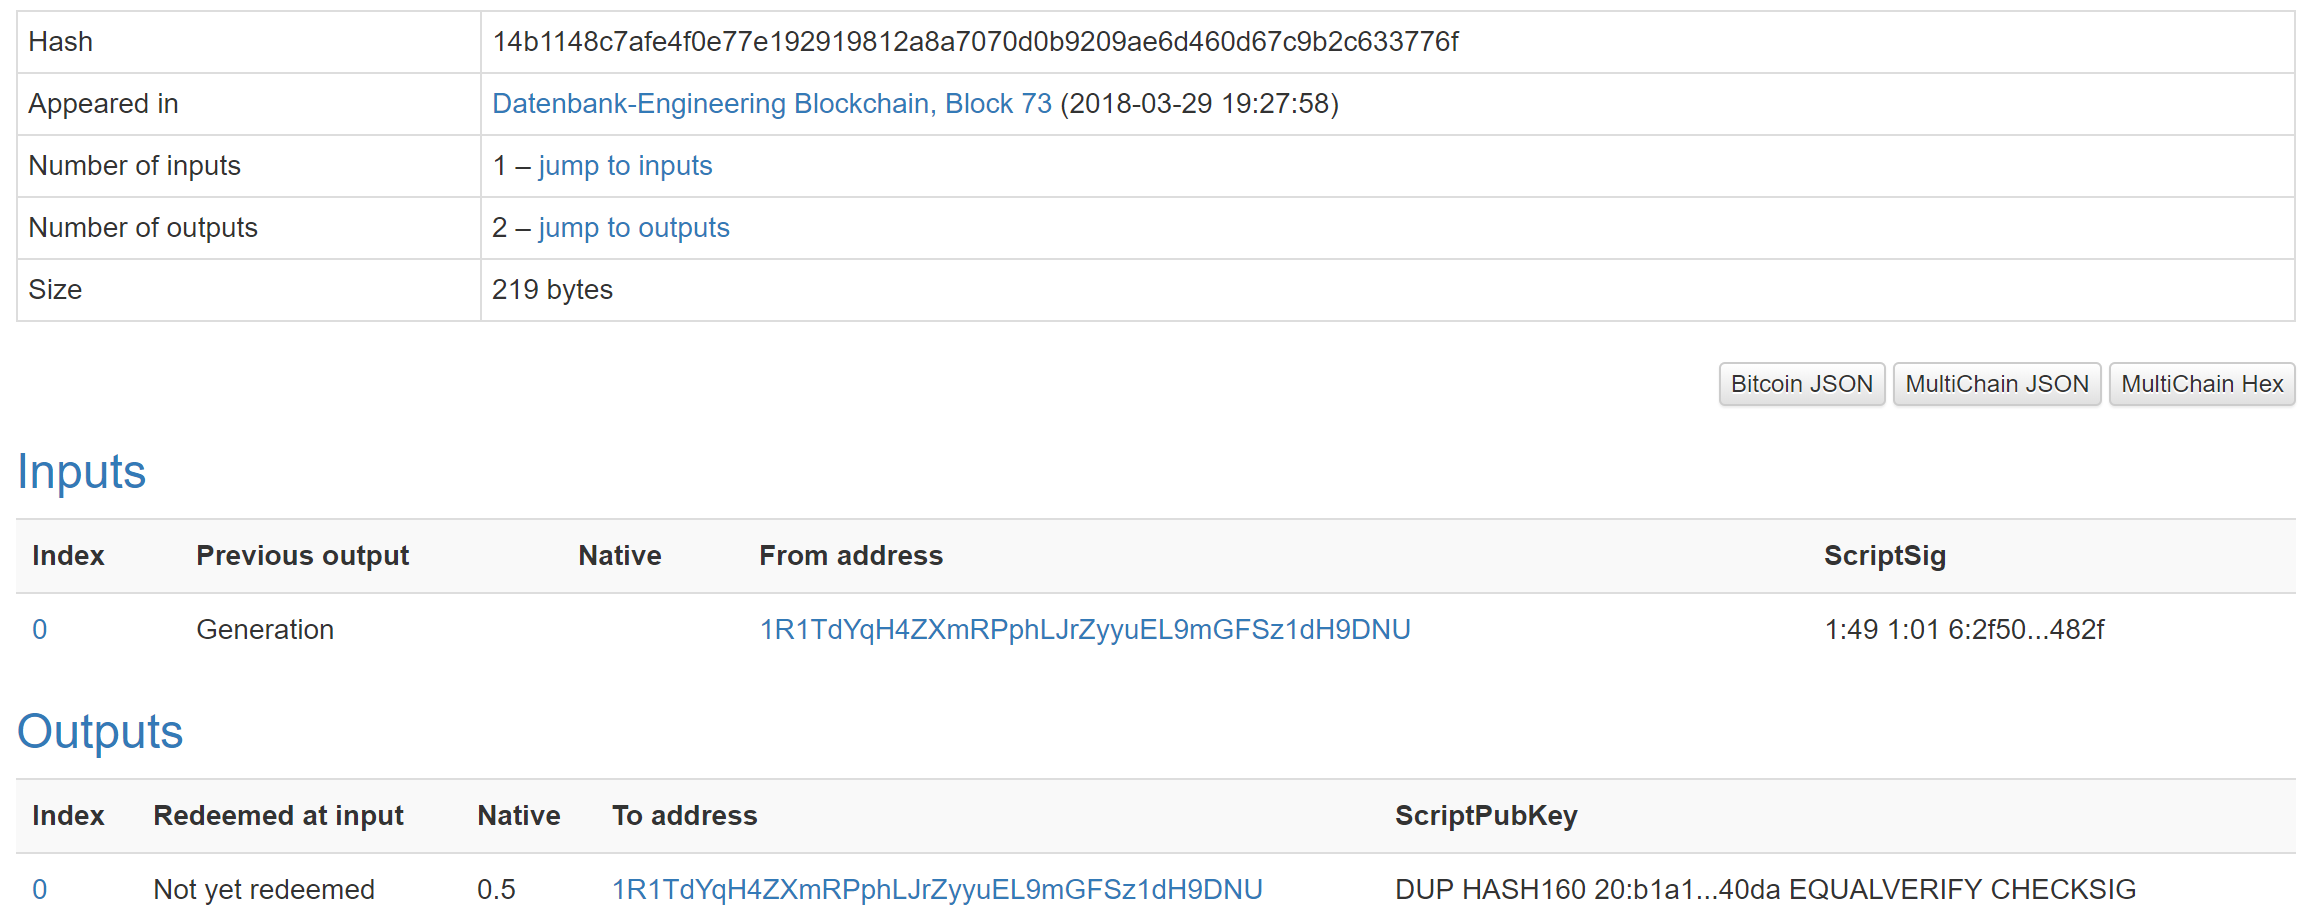
\includegraphics[width=\textwidth]{8.png}
	\caption{Detail-Ansicht einer Transaktion}
	\label{fig:8}
\end{figure}

Diese Ansicht stellt unter anderem den Hash-Wert/die ID der Transaktion, die Nummer des Blocks, in dem sie enthalten ist, und die Größe der Transaktion in Bytes dar. Außerdem sind die Inputs und Outputs der Transaktion dargestellt. Die Inputs stellen dar, wer etwas geschickt hat (From Address), wie sich die geschickte Anzahl an Währung vom Sender zusammenstellt (Native) und woher diese kommt (Previous Input). Im Output wird dargestellt, wer das Ergebnis der Transaktion erhält (To address) und wie viel Währung er erhält (Native). In Falle der abgebildeten Transaktion schickt der Server an sich selbst 0.5 Währung, die neu generiert werden (Previous Output = Generation). Dies ist die Belohnung für das erfolgreiche Validieren eines Blockes. Wird nun auf die ID eines Knotens geklickt, gelangt man zur Ansicht dessen (s. Abbildung \ref{fig:9}):

\begin{figure}[h]
	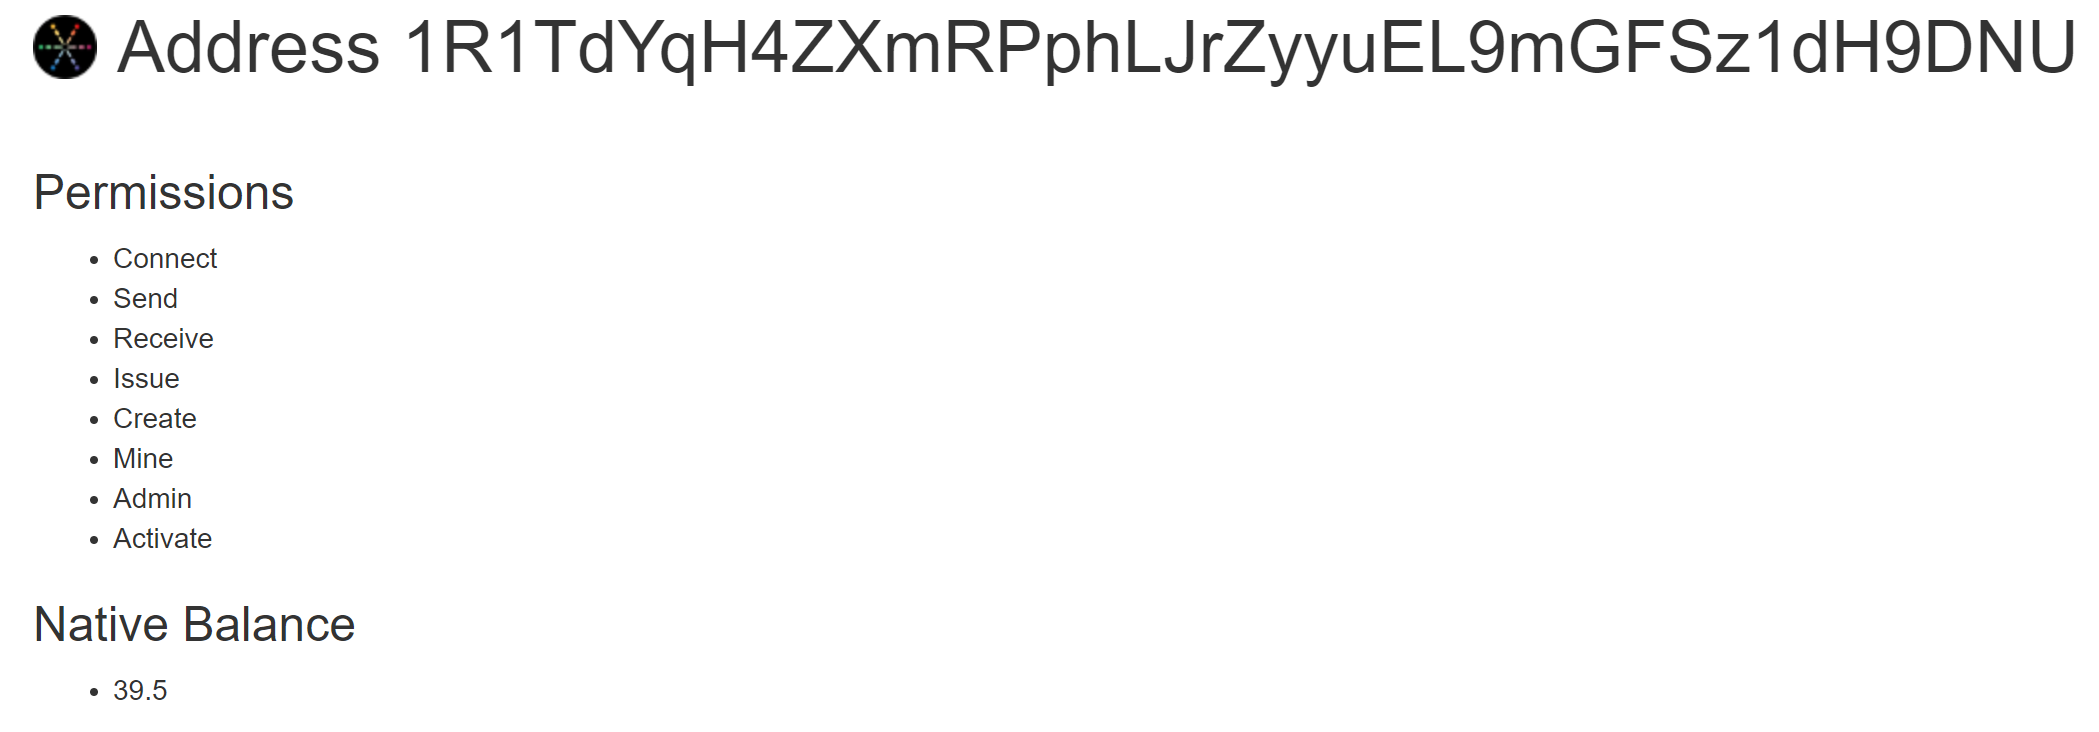
\includegraphics[width=\textwidth]{9.png}
	\caption{Explorer-Ansicht eines Knotens}
	\label{fig:9}
\end{figure}

Hier werden lediglich die Berechtigungen des Knotens (Permissions) und die Anzahl der Währung, die dieser momentan besitzt (Native Balance) aufgeführt.

\subsection{Manuelle Durchführung einer Transaktion}
Um nun eine manuelle Transaktion durchzuführen, kann man zunächst von einem Knoten zum anderen Währung überweisen. Diese Transaktion wird dann zunächst an alle Knoten der Blockchain übermittelt und dann in den nächsten Block mit aufgenommen und durch Validierung dieses Blockes gültig und durchgeführt. Um eine Transaktion von Währung durchzuführen, muss das Kommando multichain-cli gefolgt von dem Namen der Blockchain, dem Befehl send, der ID des Empfänger-Knotens und die zu überweisende Anzahl der Währung eingegeben werden. So könnte eine Überweisung des Servers an den Client wie folgt lauten:

\begin{lstlisting}[frame=single]
multichain-cli db send 18tJkQWoVaoMNWsH4CN5ruazXnLjnGPUnyAdGA 2.0
\end{lstlisting} 

Wird diese Transaktion nun durchgeführt, wird sie auf der Startseite des Explorers aufgeführt ist zunächst allerdings noch nicht bestätigt, da diese noch in keinen validierten Block mit aufgenommen wurde (s. Abbildung \ref{fig:10}).

\begin{figure}[h]
	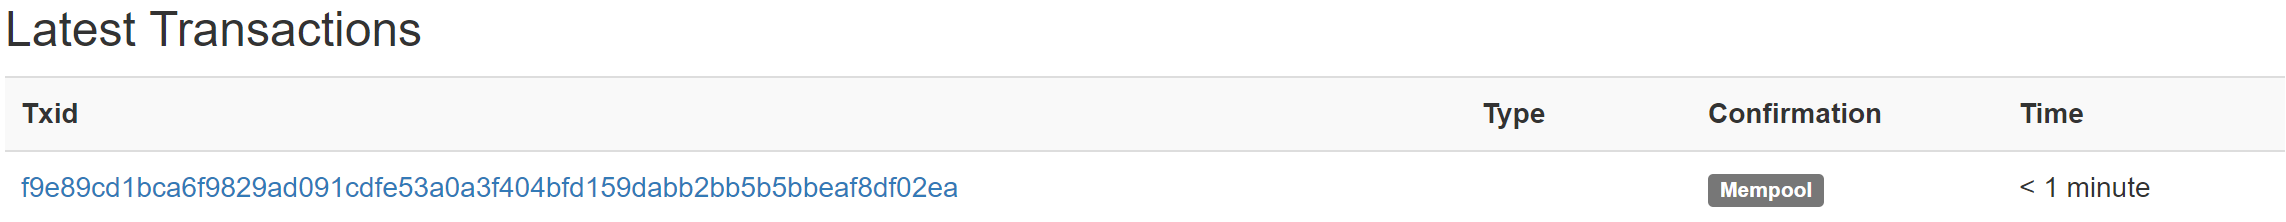
\includegraphics[width=\textwidth]{10.png}
	\caption{Unbestätigte Transaktion des Servers an den Client}
	\label{fig:10}
\end{figure}

Sobald diese Transaktion in einen validierten Block mit aufgenommen wurde, ist sie bestätigt. Wird diese Transaktion nun im Explorer betrachtet (s. nächste Abbildung), sieht man, dass der Server (From Address) viermal 0.5 Währung (Native) verschickt hat und auch aus welchen Transaktionen diese stammen (Previous Output). Dies ist dazu zurückzuführen, dass der Server bislang lediglich mehrmals 0.5 Währung durch das Validieren von Blöcken erhalten hat. Auf der Empfängerseite der Transaktion sieht man allerdings, dass der Client (To address) 2 Währung (Native) erhalten hat.

\begin{figure}[h]
	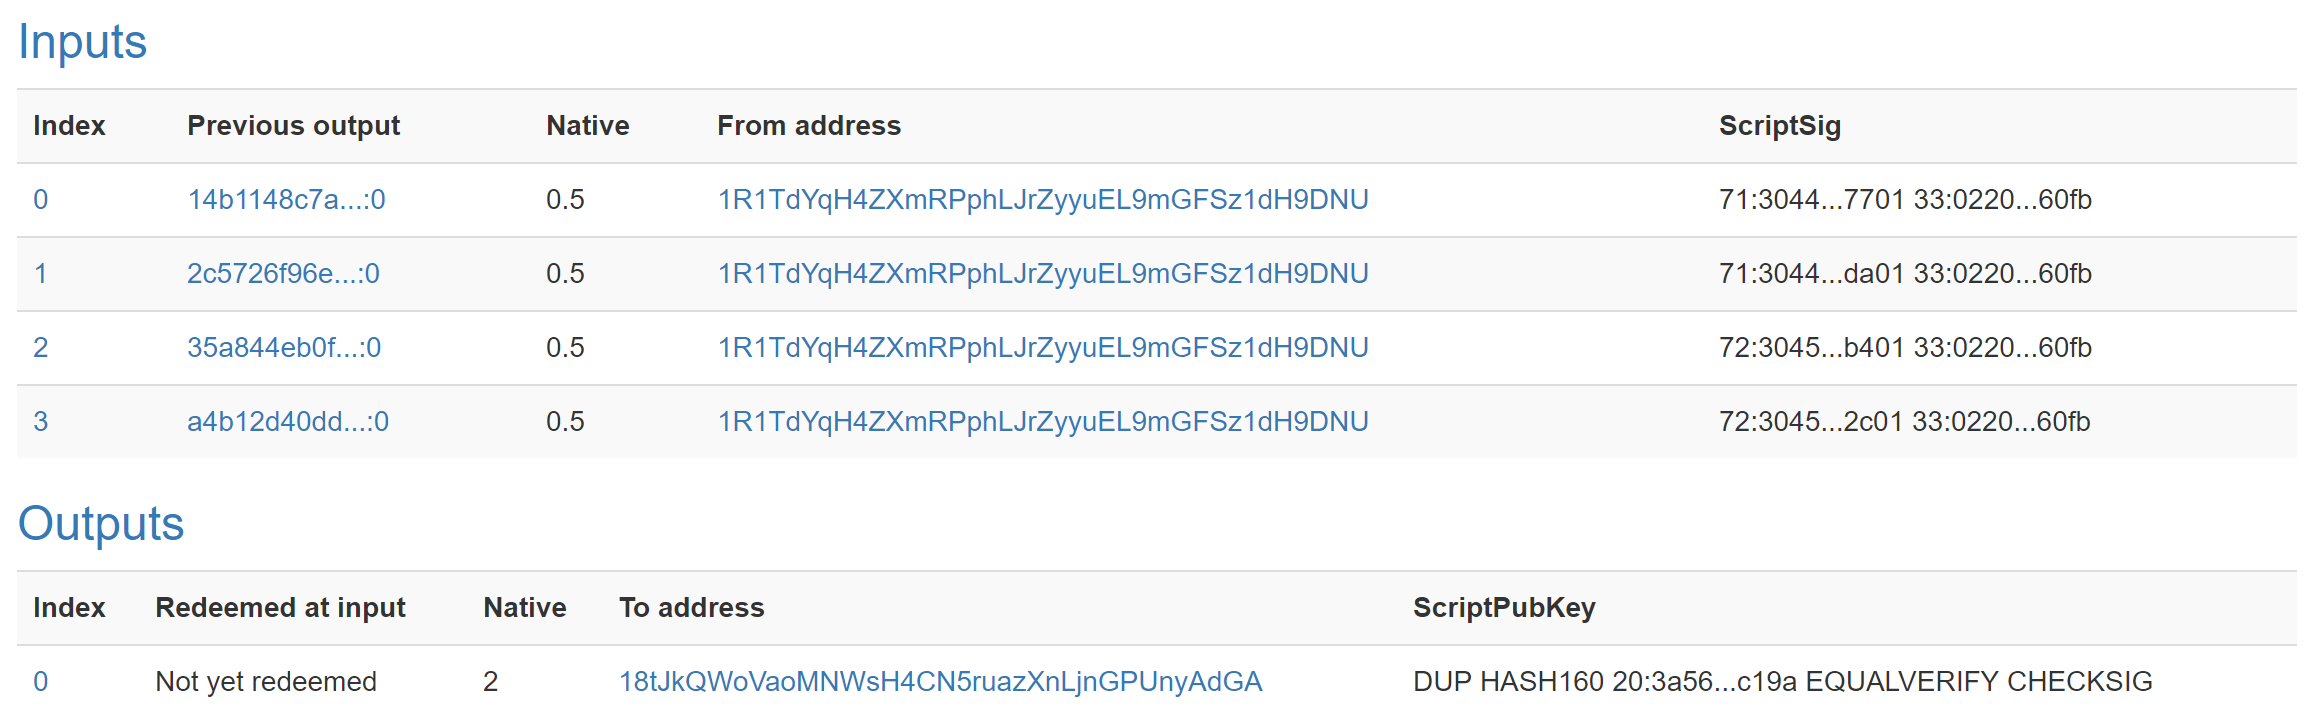
\includegraphics[width=\textwidth]{11.png}
	\caption{Betrachtung der Transaktion des Servers an den Client}
	\label{fig:11}
\end{figure}

\subsection{Speichern von Daten}
Neben dem Verschicken von Währung können in einer Blockchain allerdings auch allgemeine Daten gespeichert werden. Hierzu wird erneut auf das Kommando multichain-cli zurückgegriffen. Dabei muss erneut die Blockchain angegeben werden, gefolgt von dem Befehl publish, einem sog. Stream (root ist der Standard-Stream der Blockchain), einem Key dem die Daten zugeordnet werden sollen und mittels dem später alle Daten abgefragt werden können, die diesem Key jemals in dieser Blockchain zugeordnet wurden und den Daten selbst. Die Daten müssen allerdings im Hexadezimalformat angehängt werden. Dies hat den Vorteil, dass ganze Bilder oder Videos im hexadezimal kodierten Format an die Blockchain angehängt werden können. Ein entsprechendes Kommando könnte für diese Blockchain wie folgt aussehen:

\begin{lstlisting}[frame=single]
multichain-cli db publish key1 12345d
\end{lstlisting} 

Sobald man das Kommando bestätigt, wird eine neue Transaktion angelegt, die die Daten enthält. Die folgende Abbildung stellt diese Transaktion im Explorer dar:

\begin{figure}[h]
	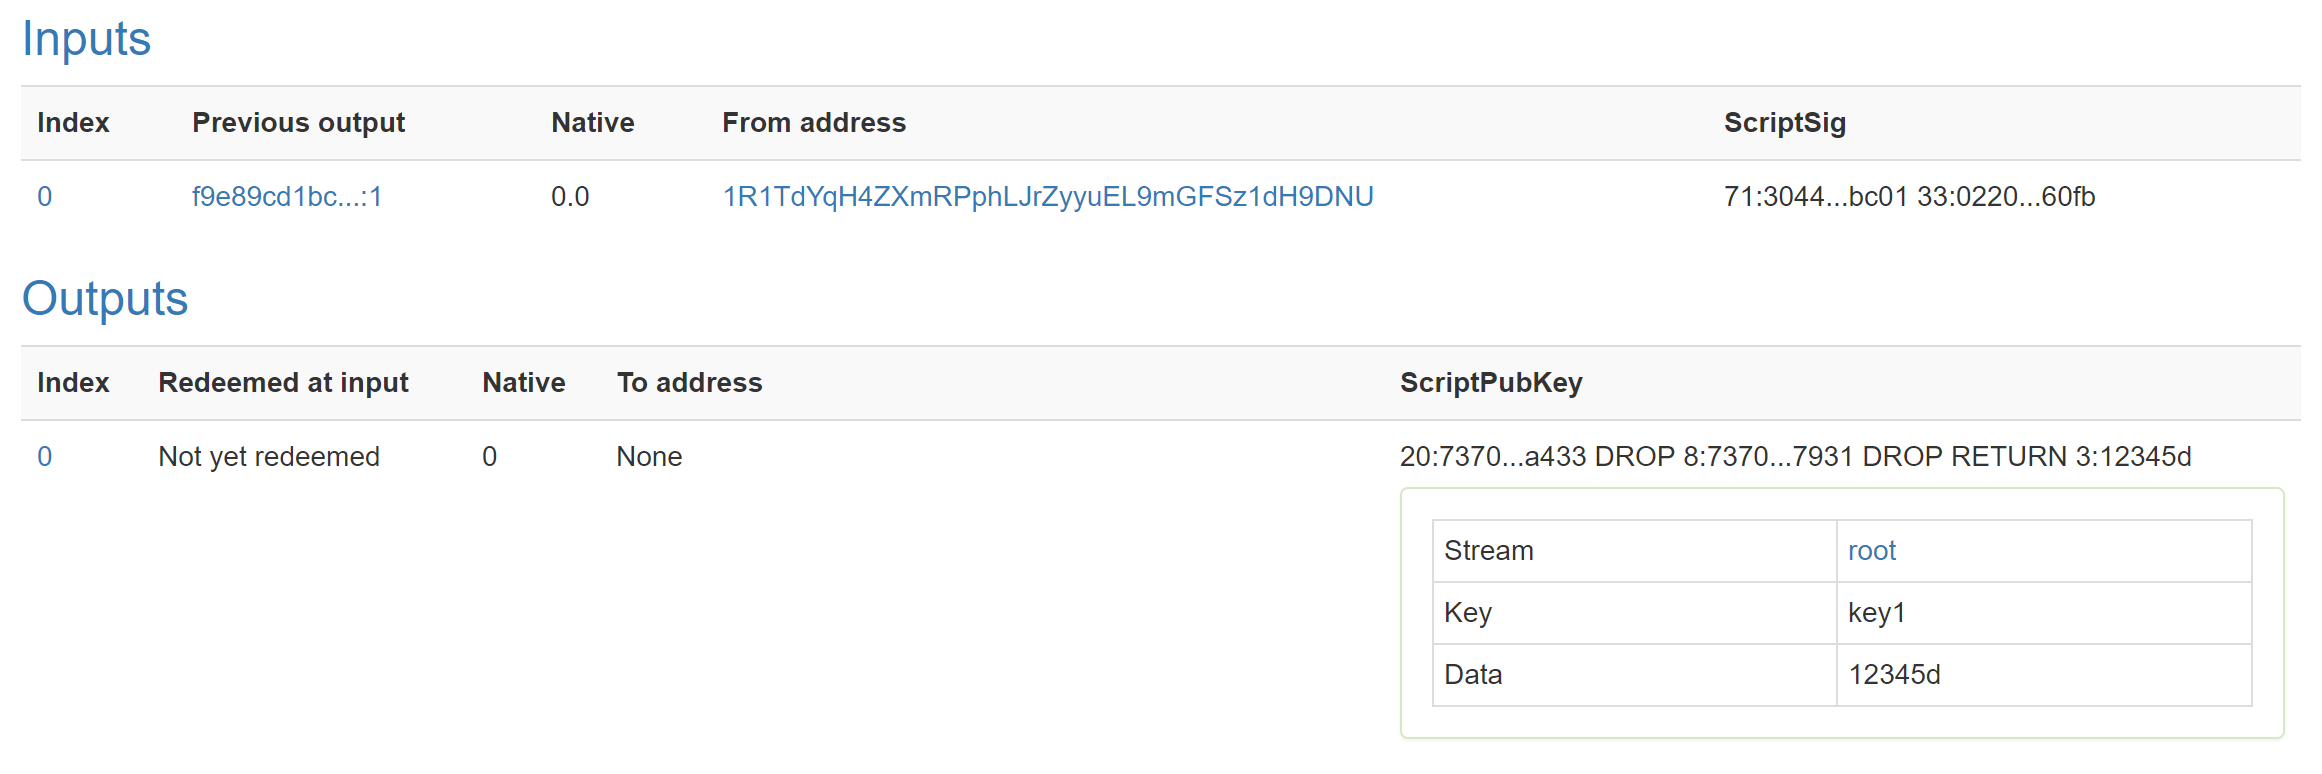
\includegraphics[width=\textwidth]{12.png}
	\caption{Transaktion im Explorer, die Daten enthält}
	\label{fig:12}
\end{figure}

Transaktionen die Daten enthalten, werden von einem Knoten (From address) in einen Stream geschrieben und an niemanden (To address) gesendet. Die Währung der Transaktion ist entsprechend 0. Beim Output der Transaktion wird allerdings eine Tabelle dargestellt, die die versendeten Daten im Feld „Data“, den Key, dem die Daten zugeordnet wurden, und den Stream, in den die Daten geschrieben wurden, enthält. Durch diese Art der Speicherung der Daten durch eine Transaktion und somit den Eingang dieser in die Merkle Root und entsprechend den Hash des validierten Blockes sind auch diese Daten kaum manipulierbar, sofern nicht alle folgenden Blöcke neu berechnet werden.